\section{Il problema}

\begin{frame}
	\sectionpage
	\centering
\end{frame}

\begin{frame}
	\frametitle{Reti complesse}
	\centering
	\begin{figure}[h]
		\centering
		\begin{flushleft}
			Grafi con caratteristiche topologiche non banali che occorrono modellando 
			
			sistemi reali (quali social network, reti neurali, computer network).
		\end{flushleft}
		\medskip
		
		\small 
		\begin{minipage}[t]{.45\textwidth}
			\centering
			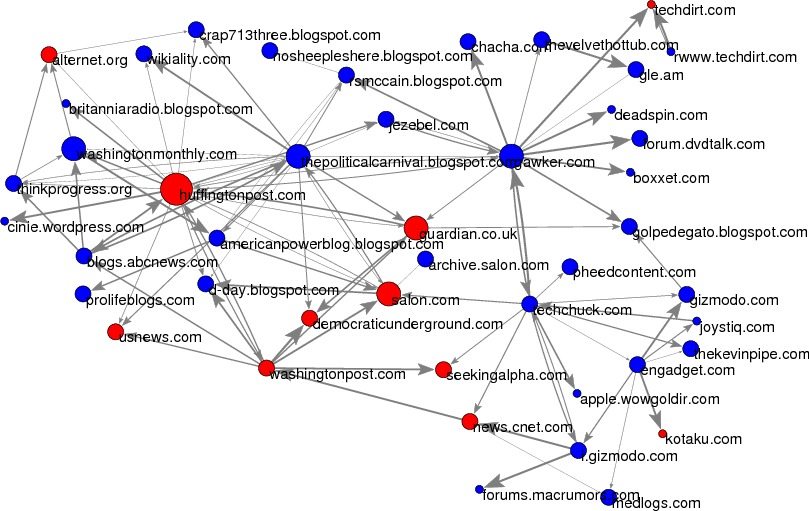
\includegraphics[width=0.9\textwidth]{images/4_netinf}
			\small 
			\caption{Diffusione delle notizie tra i vari siti e \\blog di informazione statunitensi\\ \textit{Fonte: SNAP Stanford}}
		\end{minipage}\hfill
		%\pause
		\begin{minipage}[t]{.45\textwidth}
			\centering
			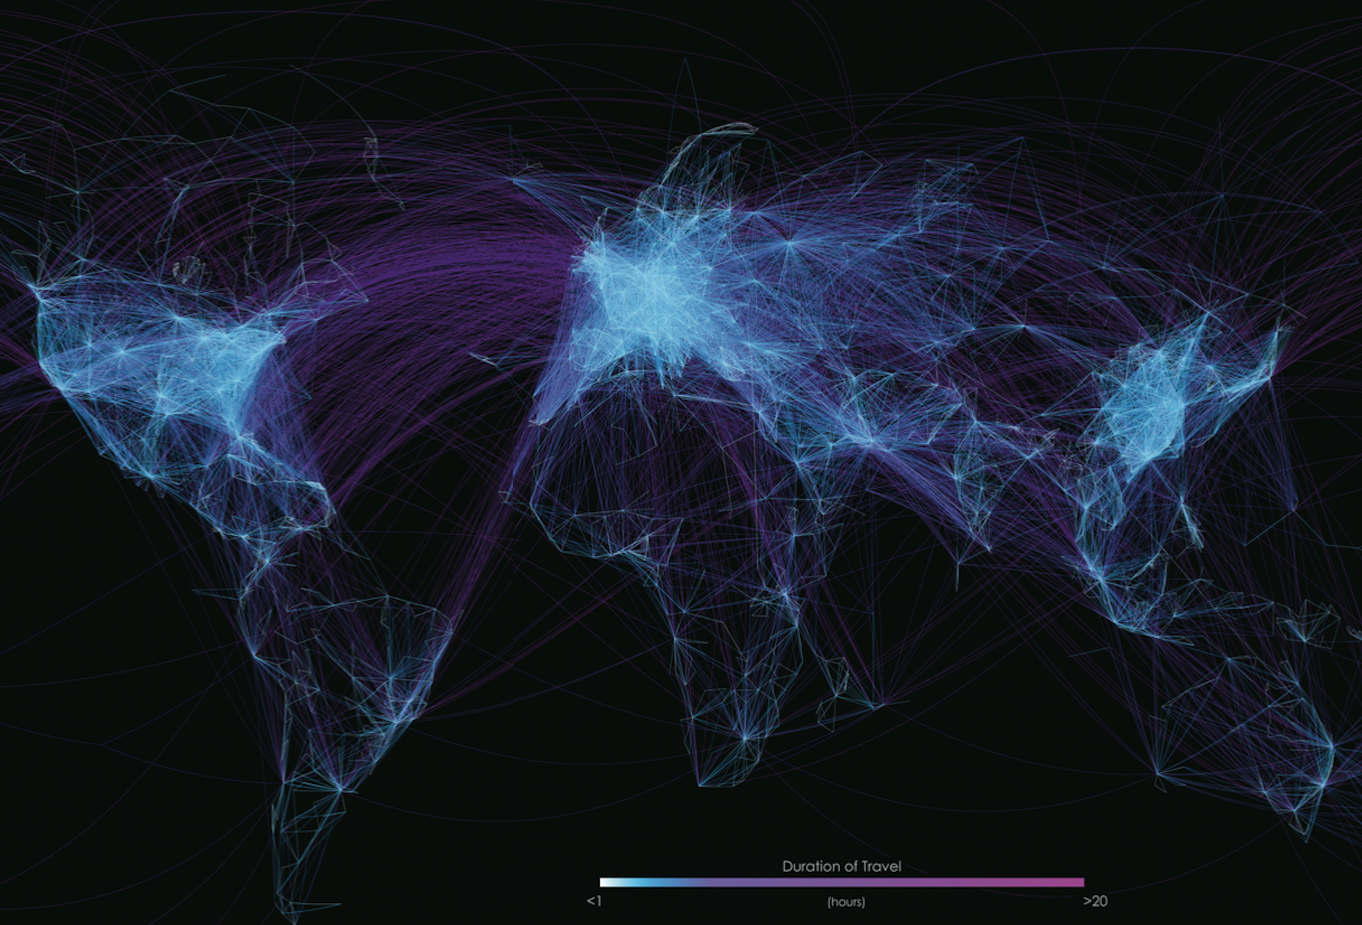
\includegraphics[width=1\textwidth]{images/7_flight}
			\small 
			\caption{Rotte dei voli commerciali  \\ \textit{Fonte: Bio Diaspora, Toronto}}
		\end{minipage}
	\end{figure}
\end{frame}

\begin{frame}
	\frametitle{Sei gradi di separazione}
	\textit{"Ho letto che ognuno di noi su questo pianeta è separato dagli altri solo da sei persone. 
		Sei gradi di separazione tra noi e tutti gli altri su questo pianeta [...]\\ una tortura cinese essere così vicini ma dover trovare sei persone giuste per il collegamento."}
	\begin{flushright}
		\small \textit{Ouisa Kittredge}, \textit{Six Degrees of Separation}
	\end{flushright}

	% \pause
	
	\begin{figure}[h]
		\centering
		\begin{minipage}[t]{.49\textwidth}
			\centering
			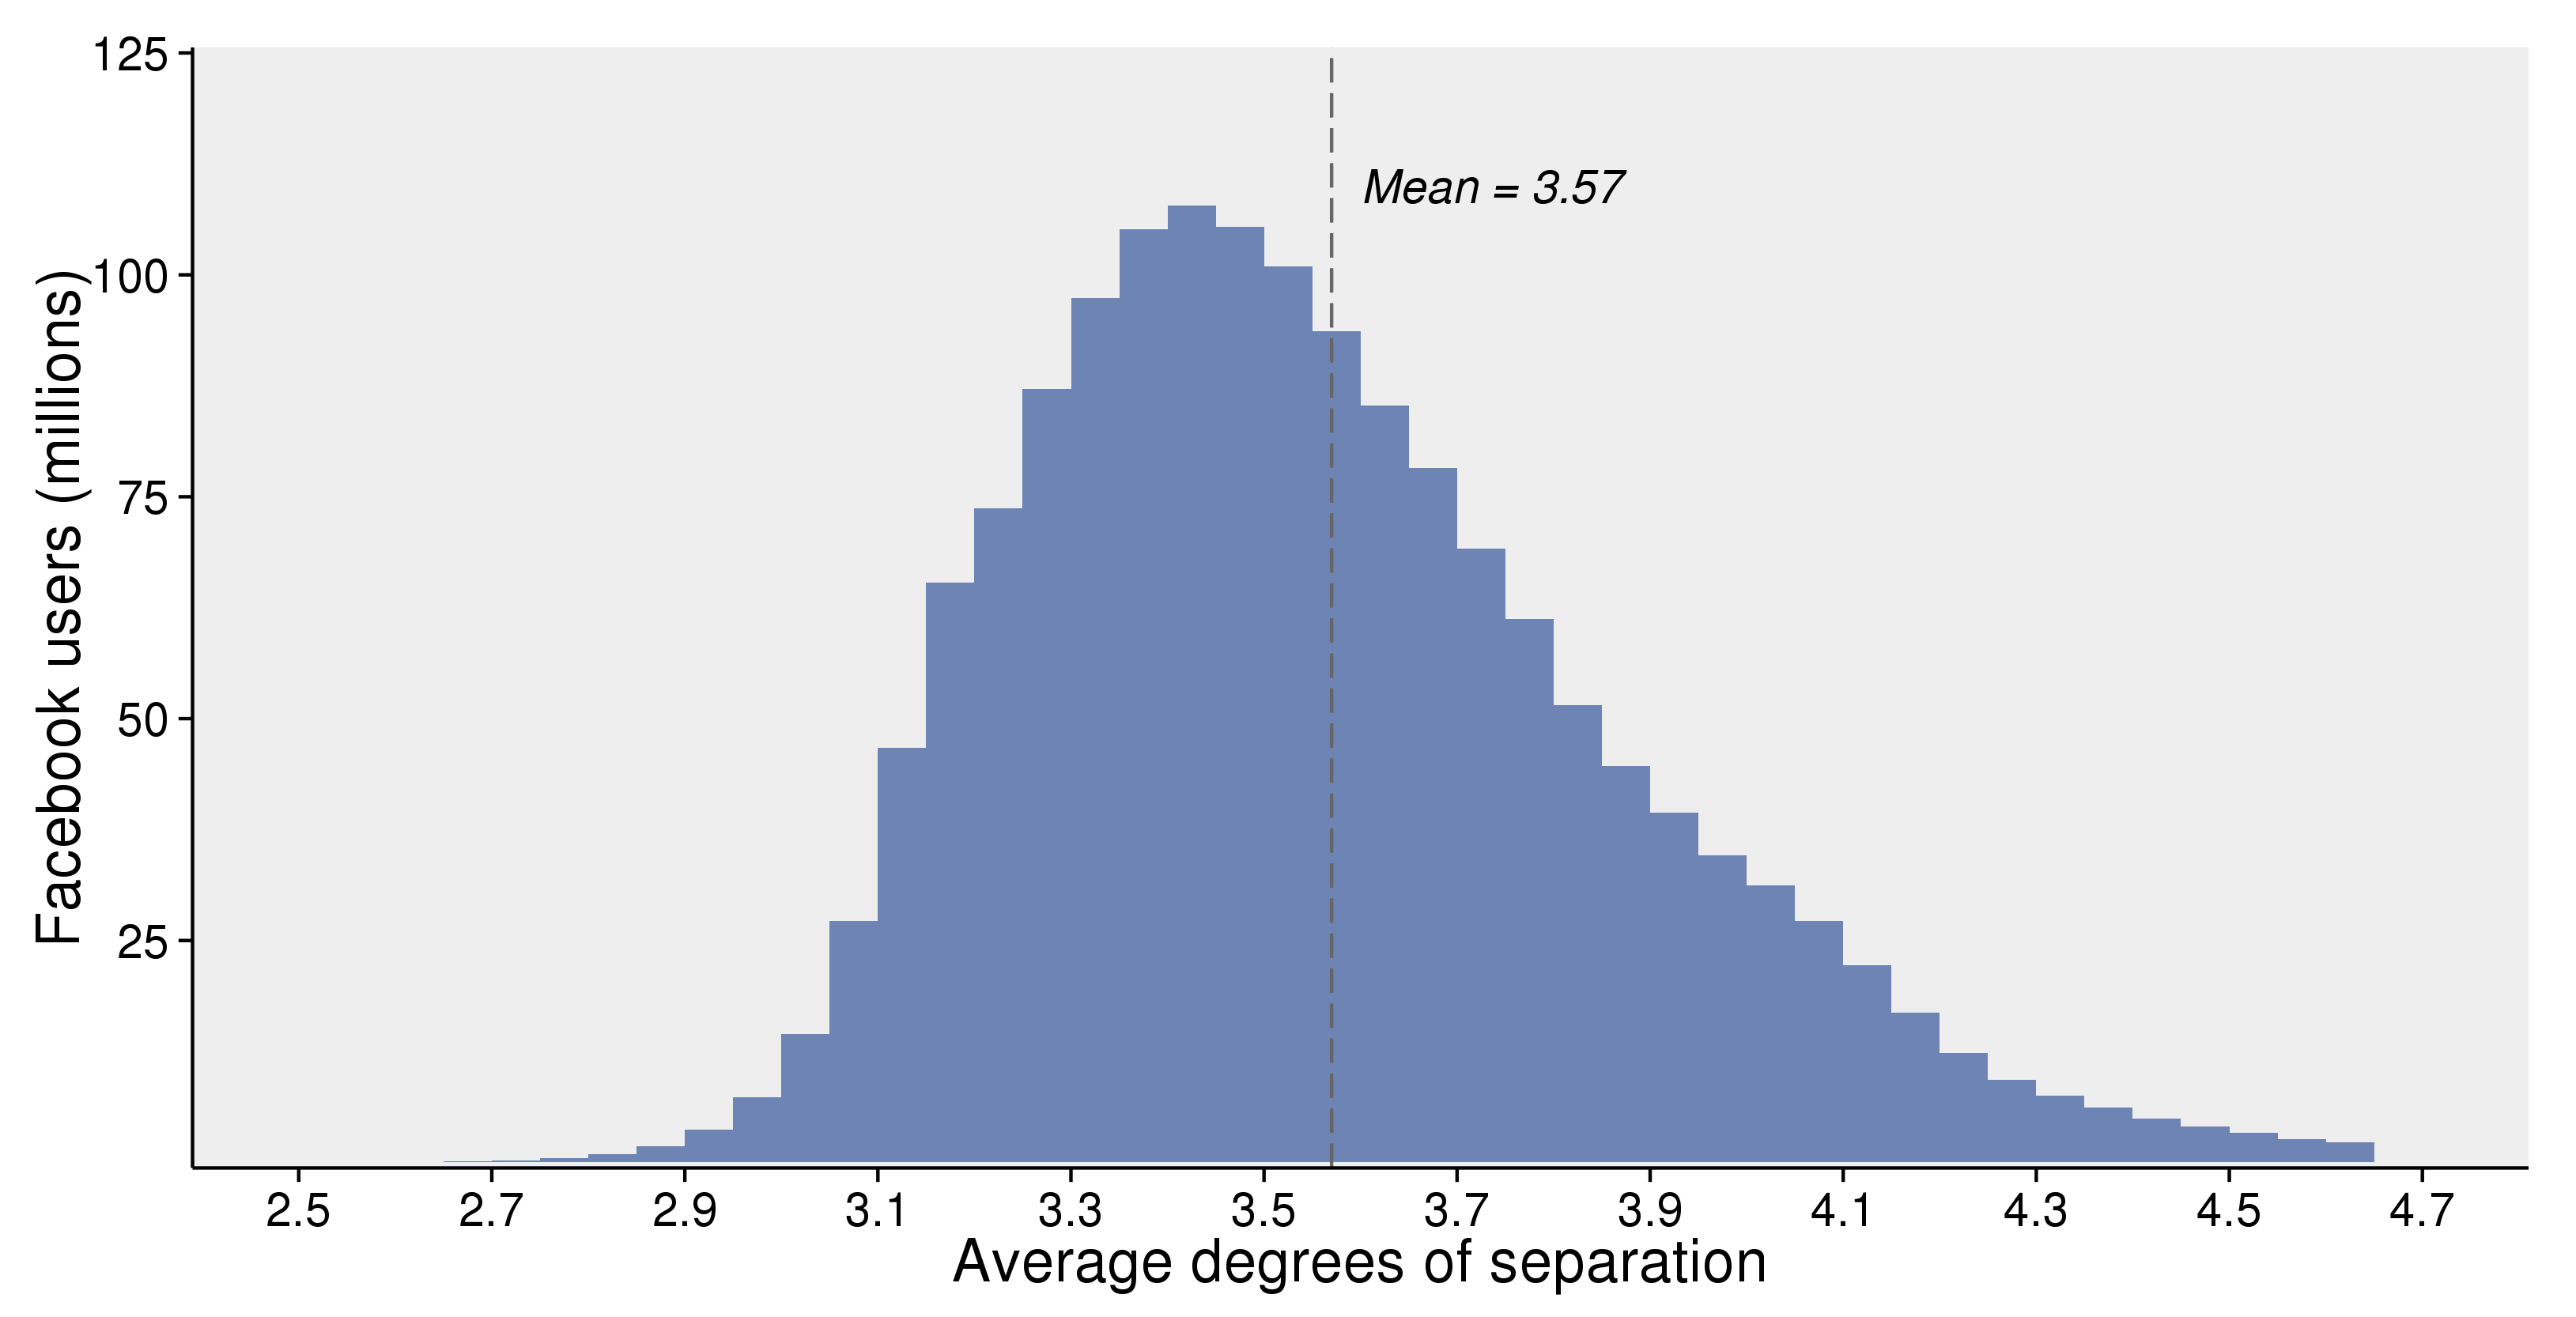
\includegraphics[width=0.9\textwidth]{images/facebook}
			\caption{In facebook la separazione media tra gli 1.6 miliardi di utenti registrati è $3.57$.\\ \textit{Fonte: facebook research, Feb 2016}}
		\end{minipage}\hfill
		%\pause
		\begin{minipage}[t]{.49\textwidth}
			\centering
			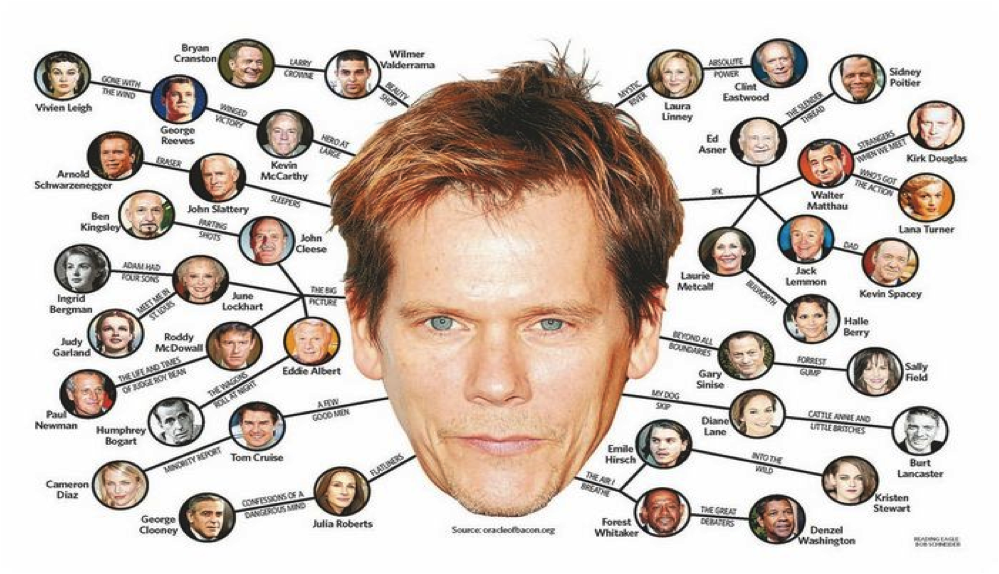
\includegraphics[width=0.9\textwidth]{images/2_kevin_bacon}
			\caption{La distanza media di collaborazioni dall'attore Kevin Bacon è $3$, il $98\%$ degli attori è a distanza minore uguale a $6$.\\ \textit{Fonte: IMDb, Ott 2017}}
		\end{minipage}
	\end{figure}
	
\end{frame}

\begin{frame}
	\frametitle{$n$-grammi e reti etichettate}
	
	\textit{"Nessun uomo è un'isola, completo in se stesso; ogni uomo è un pezzo del continente, una parte del tutto."}
	\begin{flushright}
		\small \textit{John Donne}
	\end{flushright}
	
	% \centering
	
\end{frame}

\begin{frame}
	\frametitle{Indici di similarità}
	\centering
	
	\small
	% $0 \leq J(A,B), BC(A,B) \leq 1$\\
	
	\begin{figure}[h]
		\begin{minipage}[t]{.48\textwidth}
			\centering
			\Large
			Jaccard
			\small
			\medskip
			\begin{equation*}
				J(A,B) = \frac{|A \cap B|}{|A \cup B|}
			\end{equation*}
			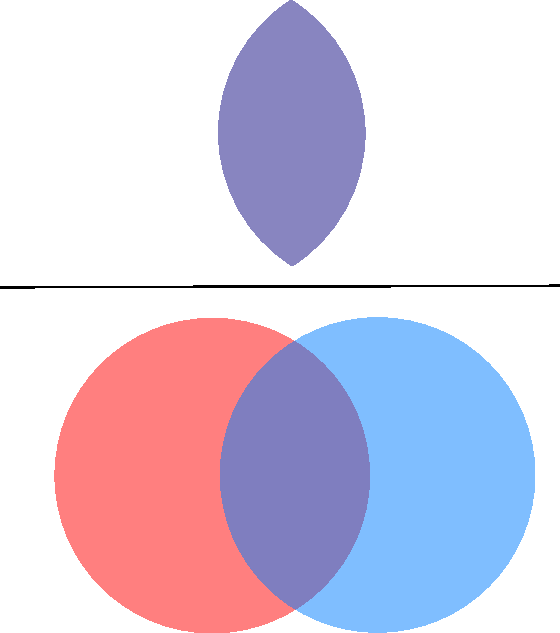
\includegraphics[width=0.5\textwidth]{images/4_jaccard}
		\end{minipage}\hfill
		%\pause
		\begin{minipage}[t]{.48\textwidth}
			\centering
			\Large
			Bray-Curtis
			\small
			\medskip
			\begin{equation*}
			BC(A,B) = \frac{2 \times |A \cap B|}{|A| + |B|}
			\end{equation*}
			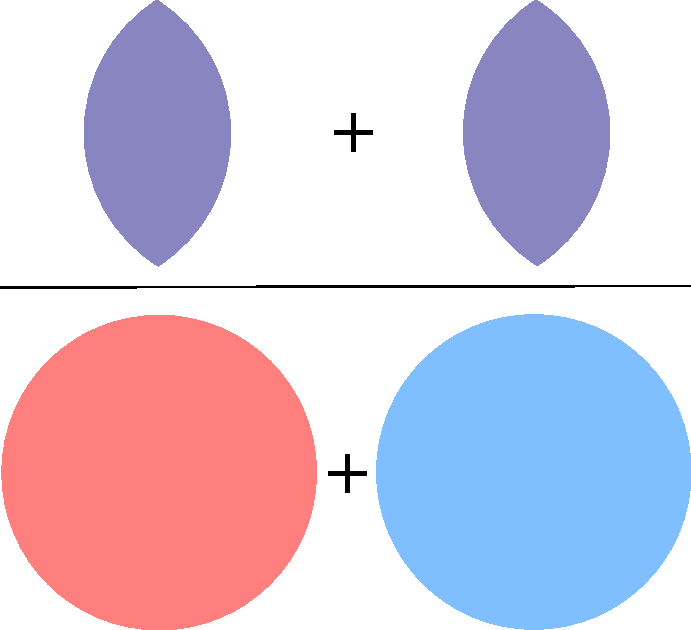
\includegraphics[width=0.6\textwidth]{images/5_bray_curtis}
			
		\end{minipage}\hfill		
	\end{figure}
	\small
	$J(A,B) = BC(A,B) = 0$ se $A \cap B = \emptyset$\medskip
	
	$J(A,B) = BC(A,B) = 1$ se $A = B$ \phantom{$\cap \emptyset.$}
	
\end{frame}

\begin{frame}
	\frametitle{Il problema}
	\centering
\end{frame}

\begin{frame}
	\frametitle{Applicazioni pratiche}
	\centering
	\begin{figure}[h]
		\centering
		\begin{minipage}[t]{.49\textwidth}
			\centering
			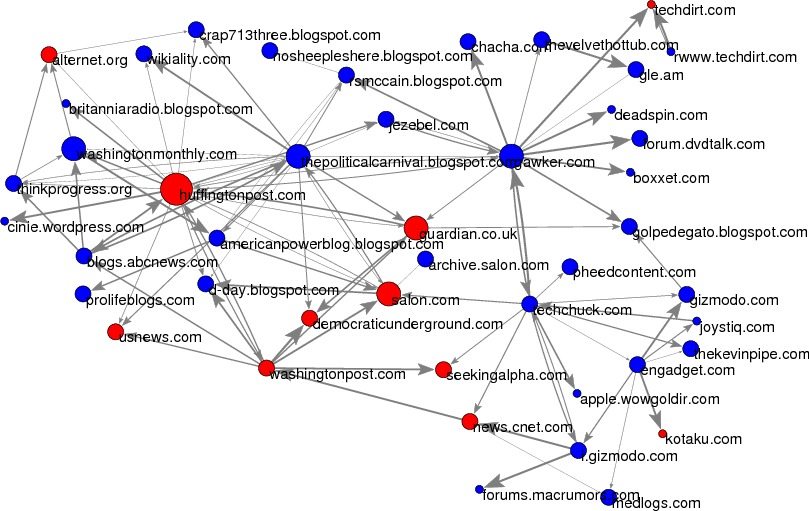
\includegraphics[width=0.9\textwidth]{images/4_netinf}
			\caption{Diffusione delle notizie tra i vari blog e siti di informazione statunitensi\\ \textit{Fonte: SNAP Stanford}}
		\end{minipage}\hfill
		%\pause
		\begin{minipage}[t]{.49\textwidth}
			\centering
			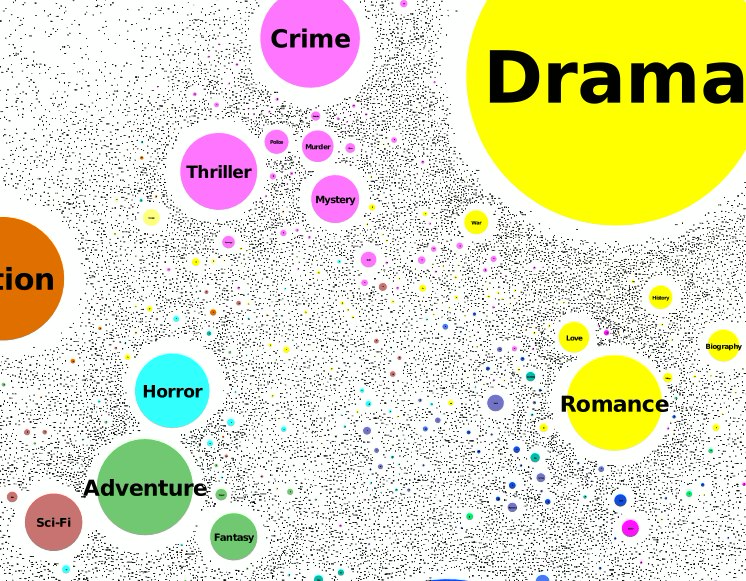
\includegraphics[width=0.9\textwidth]{images/6_imdb}
			\caption{Interazione tra i film con attori in comune\\ \textit{Fonte: IMDb}}
		\end{minipage}
	\end{figure}
\end{frame}
